\chapter{Two-source high harmonic generation}
\label{two_source}

\section{Introduction}
\label{intro_ts}

A common difficulty in working with extreme ultraviolet (XUV) light is the lack of efficient and broadband optics, especially beam splitters. In this chapter, I will introduce a method for generating two sources of XUV light by high harmonic generation using a \gls{swpg}.  This \gls{swpg} allows for the duplication of an \gls{ir} pulse, as well as precise and stable control of the relative phase between the duplicates of the input \gls{ir} pulse. The two most intense duplicates can generate harmonics which will interfere in the far-field. This can be thought of as an inline Mach-Zehnder interferometer with interferometric stability on sub-wavelength level of the high harmonic. The inherent stability of this two-source scheme will be utilized to measure both the real and imaginary parts of the refractive index of a medium.

\section{Theory}
\subsection{Laser beam shaping using diffractive optics}
\label{theory_ts}
%Describe general problem of beam shaping using DOEs. see \cite{romeroMathematicalAspectsLaser2010,romeroMathematicalTheoryLaser2010,romeroTheoryOptimalBeam2007}
%!!!!!!!!!!!!!!!!!!!!!!!!!!!!!!!!!!!!!!!!!!!!!!!!!!!!!!!!!!!!!!!!!!!!!!!!!!!!!!!!!!!!!!!!!!!!!!!!!!!!!!!!!!!!!!!!!!
%!!!!!!!!!!!!!!!!!!!!!!!!!!!!!!!!!COME BACK TO THIS SECTION LATER!!!!!!!!!!!!!!!!!!!!!!!!!!!!!!!!!!!!!!!!!!!!!!!!!!
%!!!!!!!!!!!!!!!!!!!!!!!!!!!!!!!!!!!!!!!!!!!!!!!!!!!!!!!!!!!!!!!!!!!!!!!!!!!!!!!!!!!!!!!!!!!!!!!!!!!!!!!!!!!!!!!!!!
In many experimental designs, it is advantageous to be able to shape the spatial intensity distribution of light to be something other than a typical Gaussian beam.  A common example of this is generating a beam with an approximately constant intensity across it's spatial profile (a flat-top beam).  For the experiments described herein, we will be interested in duplicating an input beam with relative phase control between the two duplicate beams.  Both of these examples are part of the general concept of laser beam shaping.  The challenge is to design an optical system such that given an input beam profile $I_{in}(x,y)$ we can generate the desired output beam profile $I_{out}(x,y)$. Ideally, this optical system is designed in such a way that it can be nearly lossless.\footnote{In the limit of geometric optics it is possible to make the optical system, in principle, lossless, however this is not generally possible when one considers the wave nature of light.}  The relevant optical system which will be used is shown in figure \ref{fig:beam_shaping_scheme}.  The system consists of a phase element which modifies the input field by $\phi(x,y)$ and a Fourier transform lens which adds a quadratic phase to the beam to focus it at the focal plane.  By appropriate choice of the phase profile of the phase element, one can produce the desired beam profile at the focal plane.


\begin{figure}
	\centering
	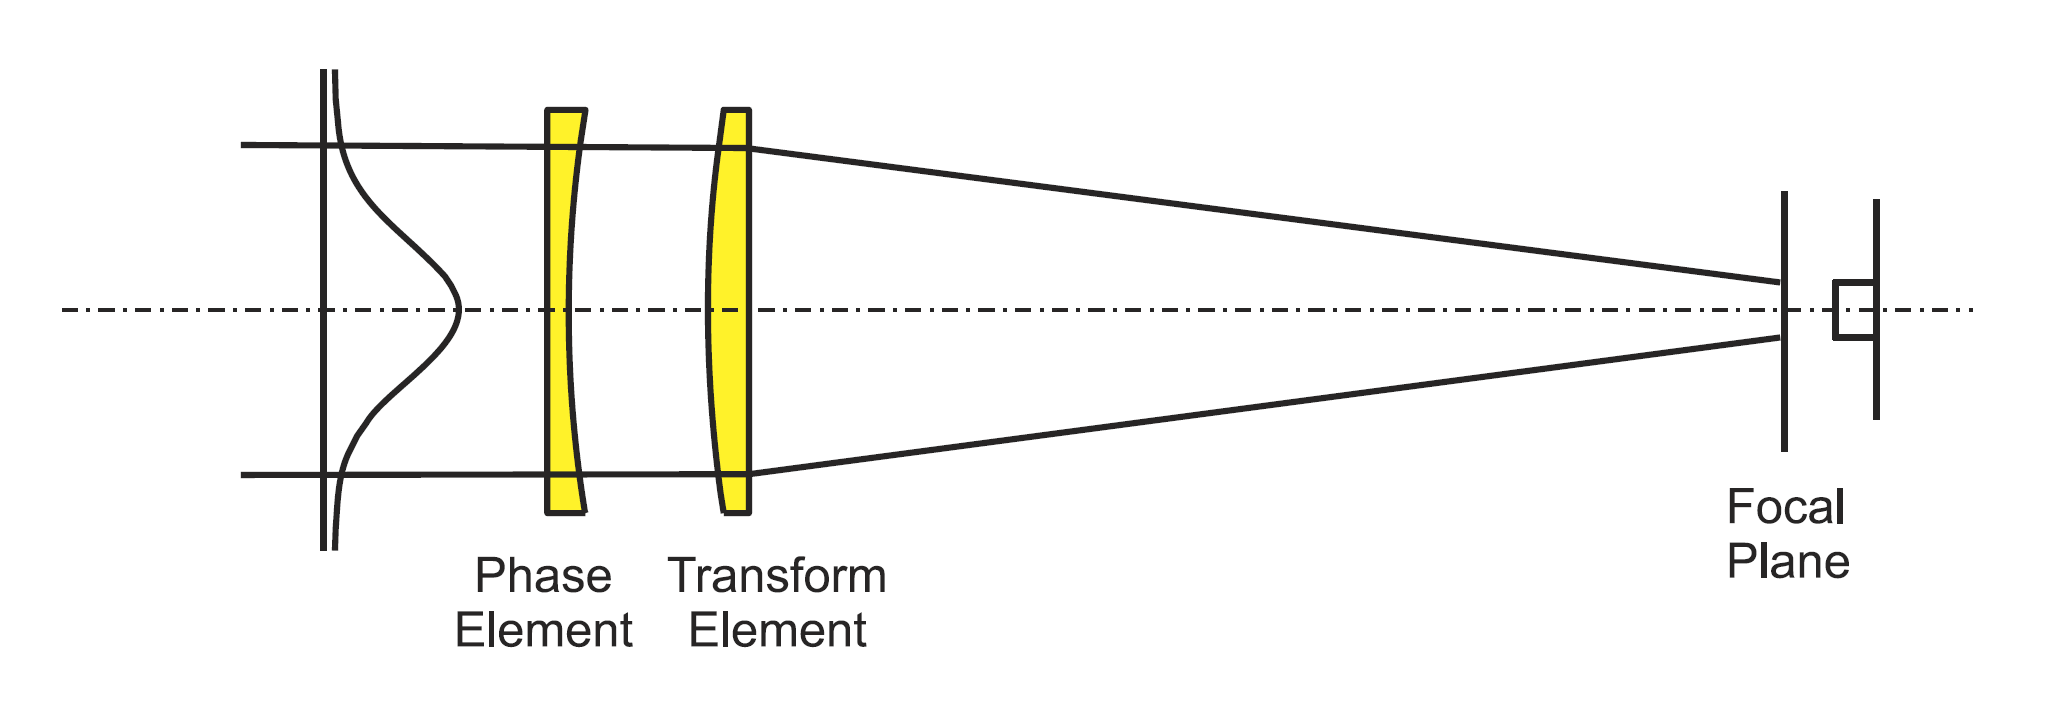
\includegraphics[width=0.9\textwidth]{figures/Two_source/romero_beam_shaping_schematic.png}
	\caption{Schematic demonstrating how to use a diffractive optical element to shape the beam profile at the focal plane. A collimated coherent beam is incident upon a diffractive optical element which shapes the phase of the incident beam, and then a lens is used as a transform element to Fourier transform the beam at the focal plane.  The intensity profile at the focal plane can be controlled by altering the spatial dependence of the phase imparted upon the incident beam by the phase element. Adapted from \cite{romeroMathematicalAspectsLaser2010}}
	\label{fig:beam_shaping_scheme}
\end{figure}


This problem can be theoretically described in terms of Fourier optics \cite{dickeyLaserBeamShaping2000, romeroMathematicalAspectsLaser2010, goodmanIntroductionFourierOptics2005}.  If one assumes that a field $u(x,y,0)$ is incident upon an an aperture at $z=0$, then the field for $z>0$ can be written under the Fresnel approximation by the Fresnel integral

\begin{equation}
\label{fresnel_integral}
	u(x,y,z)=\frac{i k}{2\pi z}e^{i k z}e^{i k (x^2+y^2)/2z}\int_{-\infty}^{\infty}\int_{-\infty}^{\infty}u(\xi,\eta,0) e^{ik(\xi^{2}+\eta^{2})/2z} e^{-ik(x\xi + y\eta)/z} \diff\xi\diff\eta
\end{equation}

where $u(\xi,\eta,0)$ is the incoming field and $k=2\pi/\lambda$ is the wavenumber.  Now, if one assumes that the phase element is placed at $z=0$, then immediately after passing through the thin phase element in Fig. \ref{fig:beam_shaping_scheme} the field is given by

\begin{equation}
	u(\xi,\eta,0)=f(\xi,\eta)e^{i\phi(\xi,\eta)}.
\end{equation} 

After propagating through the thin Fourier transform lens of focal length $f$, the field at the focal plane is now given by

\begin{equation}
\label{eqn:field_at_focus}
	u(x,y,f)=\frac{ik}{2\pi f}e^{ikf}e^{ik(x^2+y^2)/2f}\int_{-\infty}^{\infty}\int_{-\infty}^{\infty}f(\xi,\eta)e^{i\psi(\xi,\eta)}
	e^{-ik(x\xi + y\eta)/f}\diff\xi\diff\eta
\end{equation}

where

\begin{equation}
	\psi(\xi,\eta)=\phi(\xi,\eta) + k(\xi^2 + \eta^2)/2f.
\end{equation}

Now, the idea is to rewrite this field profile at the focal plane into a more intuitive form by introducing the equation

\begin{equation}
	g(\xi,\eta)=\frac{ik}{2\pi f}f(\xi,\eta)e^{i\psi(\xi,\eta)}.
\end{equation}

The Fourier transform of this function $g(\xi,\eta)$ is given by

\begin{equation}
	G(a,b)=\frac{ik}{2\pi f}\int_{-\infty}^{\infty}\int_{-\infty}^{\infty}f(\xi,\eta)e^{i\psi(\xi,\eta)}
	e^{-i(a\xi + b\eta)}\diff\xi\diff\eta.
\end{equation}

By setting $a=kx/f$ and $b=ky/f$ and taking the square complex modulus, one obtains the equation

\begin{equation}
	\rvert G(kx/f,ky/f)\rvert^{2} = \frac{k^2}{(2\pi f)^2} \bigg\rvert\int_{-\infty}^{\infty}\int_{-\infty}^{\infty}
	f(\xi,\eta)e^{i\psi(\xi,\eta)}e^{-ik(x\xi+y\eta)/f}\diff\xi\diff\eta\bigg\rvert^{2}.
\end{equation}

By comparing this equation with the square complex modulus of the field at the focal plane (equation \ref{eqn:field_at_focus}), one finds the relationship

\begin{equation}
	\rvert u(x,y,f)\rvert^2 = \rvert G(kx/f,ky/f)\rvert^2
\end{equation}

Thus, we have shown that the intensity of the field at $z=f$, $\rvert u \rvert^2$, is given by the Fourier transform of the combined phase imparted upon the incident field by both the phase element and the Fourier transform lens, $\rvert G\rvert^2$.  So, by tuning the frequency components of the phase imparted upon the beam $\phi(x,y)$, one can, in principle, produced a specific beam shape $I(x,y)$.

%add beta parameter scaling?????

\subsection{Beam splitting grating}
\subsection{Imperfect phase grating}
\section{Two-source high harmonic generation}


\begin{equation}
\label{eq:field}
S(x) = \sum_{n} E(x - x_{n})
\end{equation}






\begin{figure}
	\centering
	\begin{subfigure}[b]{0.45\textwidth}
		\caption{}
		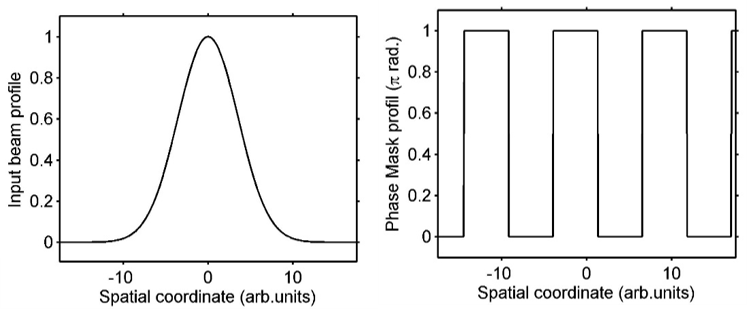
\includegraphics[width=\textwidth]{figures/Two_source/spatial_profile}
		\label{fig:spatial_profile}
	\end{subfigure}
	\begin{subfigure}[b]{0.45\textwidth}
		\caption{}
		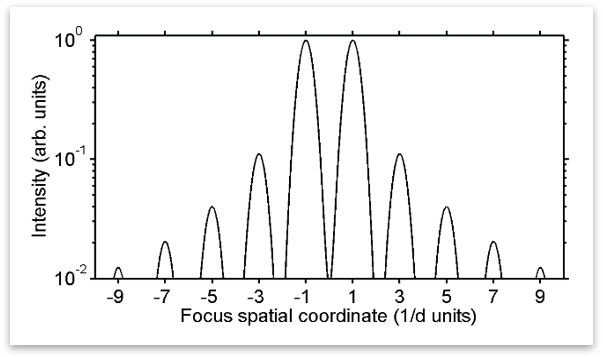
\includegraphics[width=\textwidth]{figures/Two_source/focus_profile}
		\label{fig:focus_profile}
	\end{subfigure}
	\caption{(a) Two-channel model for Feshbach resonance.  Incident atoms in the entrance channel (the open channel) couple to a bound state of energy $E_{c}$ supported by the closed channel.  Since collisions take place for $E\rightarrow 0$, tuning $E_{c}$ to 0 allows for the resonant coupling to occur. (b) Scattering length near a resonance where a bound state crosses the scattering threshold. Inset shows the quadratic behavior of the binding energy near the resonance.}
\end{figure}


\begin{equation}
	\begin{aligned}
    	I_{IR} &= a + b\times\cos\left(\phi(x_{0})\right)\\
     	I_{q} &= \alpha_q\times a^{q} \left(1+N_{q}\frac{b}{a}\cos\left(\phi(x_{0})\right)\right) + o(b\times a^{q-1})\\
	\end{aligned}
\end{equation}
\begin{equation}
	\begin{aligned}
		I_{IR}(\tilde{x}_{1},x_{0}) &= \left|\tilde{S}(\tilde{x}_{1},x_{0})\right|^{2} \\
		&= \left|a_{-1}\tilde{E}(2\tilde{x}_{1})+a_{0}\tilde{E}(\tilde{x}_{1})+a_{1}\tilde{E}(0)+a_{3}\tilde{E}(2\tilde{x}_{1})\right|^{2}\\
     &= \left|a_{0}\tilde{E}(\tilde{x}_{1})+a_{1}\tilde{E}(0)\right|^{2}\\
	\end{aligned}
\end{equation}
\begin{equation}
	\begin{aligned}
		 I_{IR}(\tilde{x}_{1},x_{0}) &=\left|\tilde{E}(0)\right|^{2}\left|\frac{2}{\pi}\sin\left(\xi\frac{\pi}{2}\right)e^{i(\xi\frac{\pi}{2}-\phi_{1})}+\cos\left(\xi\frac{\pi}{2}\right)e^{i\xi\frac{\pi}{2}}\frac{\tilde{E}(\tilde{x}_{1})}{\tilde{E}(0)} -  \frac{2\sin\left(\xi\frac{\pi}{2}\right)}{\pi}e^{i(\xi\frac{\pi}{2}+\phi_{1})}\frac{\tilde{E}(2\tilde{x}_{1})}{\tilde{E}(0)} + \frac{2\sin\left(\xi\frac{\pi}{2}\right)}{3\pi}e^{i(\xi\frac{\pi}{2}-3\phi_{1})}\frac{\tilde{E}(2\tilde{x}_{1})}{\tilde{E}(0)}\right|^{2}\\
	\end{aligned}
\end{equation}
\begin{equation}
	\begin{aligned}
		I_{IR}(\tilde{x}_{1},x_{0})  &= \left|\tilde{E}(0)\frac{2}{\pi}\sin\left(\xi\frac{\pi}{2}\right)\right|^{2}\left|e^{-i\phi_{1}}+\frac{\pi}{2\tan\left(\xi\frac{\pi}{2}\right)}\frac{\tilde{E}(\tilde{x}_{1})}{\tilde{E}(0)} -e^{i\phi_{1}}\frac{\tilde{E}(2\tilde{x}_{1})}{\tilde{E}(0)} +  \frac{e^{-3i\phi_{1}}}{3}\frac{\tilde{E}(2\tilde{x}_{1})}{\tilde{E}(0)}\right|^{2}\\
		&= \left|\tilde{E}(0)\frac{2}{\pi}\sin\left(\xi\frac{\pi}{2}\right)\right|^{2}\left(1+\frac{\pi}{\tan\left(\xi\frac{\pi}{2}\right)}\frac{\tilde{E}(\tilde{x}_{1})}{\tilde{E}(0)}\cos(\phi_{1})-\frac{4}{3}\frac{\tilde{E}(2\tilde{x}_{1})}{\tilde{E}(0)}\cos(2\phi_{1})\right)\\
		I_{IR}(\tilde{x}_{-1},x_{0}) &= \left|\tilde{S}(\tilde{x}_{-1},x_{0})\right|^{2} \\
		 &= \left|a_{-1}\tilde{E}(0)+a_{0}\tilde{E}(\tilde{x}_{1})\right|^{2}\\
		&= \left|\tilde{E}(0)\right|^{2}\left|-\frac{2}{\pi}\sin\left(\xi\frac{\pi}{2}\right)e^{i(\xi\frac{\pi}{2}+\phi_{1})}+\cos\left(\xi\frac{\pi}{2}\right)e^{i\xi\frac{\pi}{2}}\frac{\tilde{E}(\tilde{x}_{1})}{\tilde{E}(0)}+\frac{2\sin\left(\xi\frac{\pi}{2}\right)}{\pi}e^{(\xi\frac{\pi}{2}-\phi_{1})}\frac{\tilde{E}(2\tilde{x}_{1})}{\tilde{E}(0)} -  \frac{2\sin\left(\xi\frac{\pi}{2}\right)}{3\pi}e^{(\xi\frac{\pi}{2}+3\phi_{1})}\frac{\tilde{E}(2\tilde{x}_{1})}{\tilde{E}(0)}\right|^{2}\\
      &= \left|\tilde{E}(0)\frac{2}{\pi}\sin\left(\xi\frac{\pi}{2}\right)\right|^{2}\left|e^{-i\phi_{1}}-\frac{\pi}{2\tan\left(\xi\frac{\pi}{2}\right)}\frac{\tilde{E}(\tilde{x}_{1})}{\tilde{E}(0)} -e^{i\phi_{1}}\frac{\tilde{E}(2\tilde{x}_{1})}{\tilde{E}(0)} +  \frac{e^{-3i\phi_{1}}}{3}\frac{\tilde{E}(2\tilde{x}_{1})}{\tilde{E}(0)}\right|^{2}\\
      &= \left|\tilde{E}(0)\frac{2}{\pi}\sin\left(\xi\frac{\pi}{2}\right)\right|^{2}\left(1-\frac{\pi}{\tan\left(\xi\frac{\pi}{2}\right)}\frac{\tilde{E}(\tilde{x}_{1})}{\tilde{E}(0)}\cos(\phi_{1})-\frac{4}{3}\frac{\tilde{E}(2\tilde{x}_{1})}{\tilde{E}(0)}\cos(2\phi_{1})\right)\\
      %\forall n \in \mathbb{Z}, a^{\xi}_{2n+1}(x_{0}) &= \frac{2\sin\left(\xi\frac{\pi}{2}\right)}{(2n+1)\pi}e^{i(\xi\frac{\pi}{2}-(2n+1)\phi_{1})} \\
     a^{\xi}_{0}(x_{0}) &= \cos\left(\xi\frac{\pi}{2}\right)e^{i\xi\frac{\pi}{2}}
     \end{aligned}
\end{equation}


\begin{figure}
	\centering
	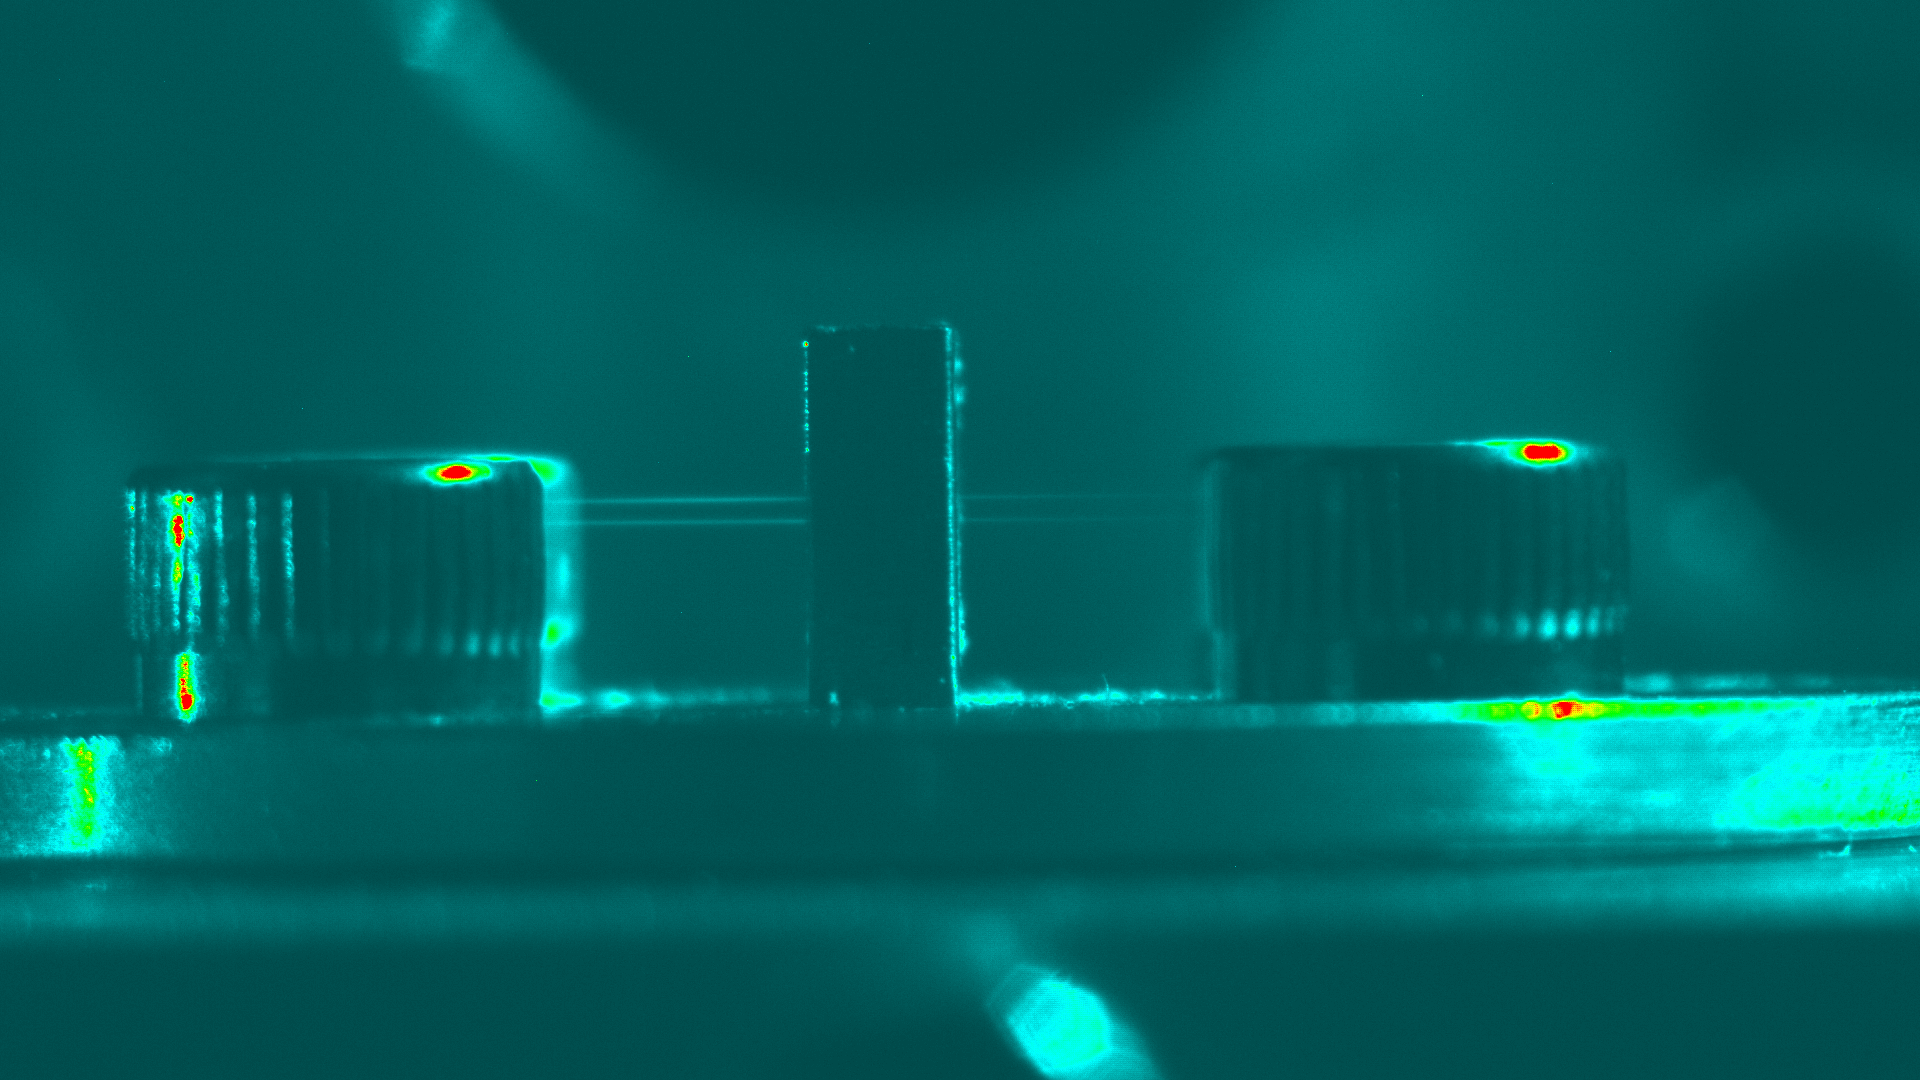
\includegraphics[width=0.9\textwidth]{figures/Two_source/ts_filament_gas_cell.png}
	\caption{Camera image of two sources generating a filament in a gas cell. Image was taken while chamber was vented and at ambient pressure.}
	\label{ts_filament}
\end{figure}

%\lipsum

\begin{figure}
	\centering
	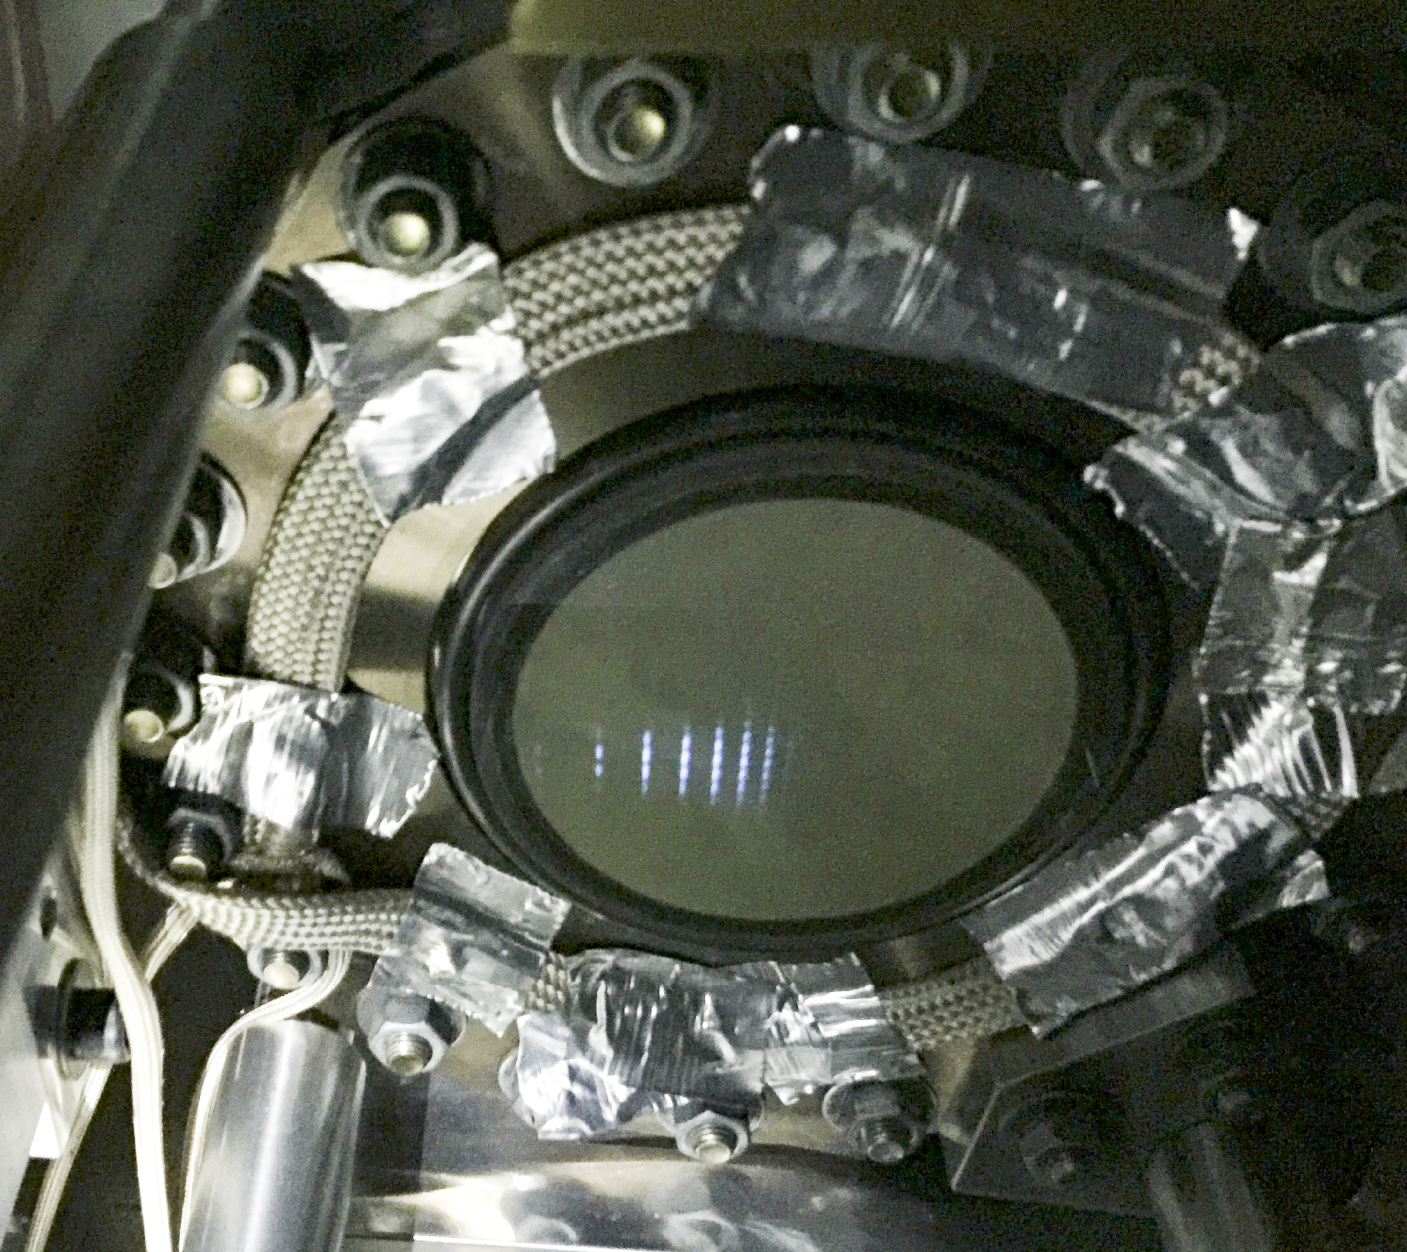
\includegraphics[width=0.9\textwidth]{figures/Two_source/MCP_ts_harmonics.png}
	\caption{Camera image of the output of the phosphor screen.  Harmonics are visible by eye.}
	\label{MCP_ts_harmonics}
\end{figure}


%\lipsum